% !TeX program = xelatex
\documentclass[a4paper,10pt]{article}

% ============================================================================
% កញ្ចប់បណ្ណាល័យ (Packages) – តាមលំនាំ NGS Preah Krasang (ls_plan.tex)
% ============================================================================
\usepackage[a4paper, left=0.95cm, right=0.95cm, top=0.85cm, bottom=0.92cm, footskip=0.52cm]{geometry}
\usepackage{amsmath, amssymb}
\usepackage{unicode-math}
\usepackage{fontspec}
\usepackage{array, longtable, multirow, colortbl}
\usepackage[table]{xcolor}
\usepackage{enumitem}
\usepackage{pifont}
\usepackage{fancyhdr}
\usepackage{tikz}
\usetikzlibrary{calc, arrows.meta, positioning, decorations.markings, babel}

% LaTeX 2025 + longtable v4.24 compatibility guard
\makeatletter
\let\@expl@@@mark@update@singlecol@structures@@\relax
\makeatother

% ============================================================================
% ការកំណត់ពុម្ពអក្សរ (Fonts Configuration - Cross-Platform Windows + Cloud fonts/)
% ============================================================================
\providecommand{\NGSFindFonts}{%
  \IfFileExists{C:/Windows/Fonts/cambria.ttc}{%
    \def\NGSSysPath{C:/Windows/Fonts/}%
    \def\NGSUserPath{C:/Users/KIT/AppData/Local/Microsoft/Windows/Fonts/}%
  }{%
    \IfFileExists{./fonts/KhmerOSsiemreap.ttf}{\def\NGSSysPath{./fonts/}\def\NGSUserPath{./fonts/}}{%
    \IfFileExists{../fonts/KhmerOSsiemreap.ttf}{\def\NGSSysPath{../fonts/}\def\NGSUserPath{../fonts/}}{%
    \IfFileExists{../../fonts/KhmerOSsiemreap.ttf}{\def\NGSSysPath{../../fonts/}\def\NGSUserPath{../../fonts/}}{%
    \IfFileExists{../../../fonts/KhmerOSsiemreap.ttf}{\def\NGSSysPath{../../../fonts/}\def\NGSUserPath{../../../fonts/}}{%
    \IfFileExists{../../../../fonts/KhmerOSsiemreap.ttf}{\def\NGSSysPath{../../../../fonts/}\def\NGSUserPath{../../../../fonts/}}{%
    \IfFileExists{../../../../../fonts/KhmerOSsiemreap.ttf}{\def\NGSSysPath{../../../../../fonts/}\def\NGSUserPath{../../../../../fonts/}}{%
    \IfFileExists{../../../../../../fonts/KhmerOSsiemreap.ttf}{\def\NGSSysPath{../../../../../../fonts/}\def\NGSUserPath{../../../../../../fonts/}}{%
      \def\NGSSysPath{../../../../../../../fonts/}\def\NGSUserPath{../../../../../../../fonts/}%
    }}}}}}}%
  }%
}
\NGSFindFonts

\setmathfont[
  Path={\NGSSysPath},
  FontIndex=1,
  Scale=1.02
]{cambria.ttc}

\defaultfontfeatures{Ligatures=TeX}

\setmainfont[
  Path={\NGSUserPath},
  Extension=.ttf,
  Script=Khmer,
  BoldFont={KhmerOSsiemreap},
  BoldFeatures={FakeBold=1.8},
  ItalicFont={KhmerOSsiemreap},
  ItalicFeatures={FakeSlant=0.25},
  BoldItalicFont={KhmerOSsiemreap},
  BoldItalicFeatures={FakeBold=1.8, FakeSlant=0.25}
]{KhmerOSsiemreap}

% ហាមដាក់ FakeBold លើ KhmerOSmuollight និងត្រូវរុំអក្សរឡាតាំង/លេខ ASCII ក្នុង \enbf{...}
\newfontfamily\muol[
  Path={\NGSUserPath},
  Extension=.ttf,
  Script=Khmer
]{KhmerOSmuollight}

\newfontfamily\TimesEn[
  Path={\NGSSysPath},
  Extension=.ttf,
  Scale=1.00,
  BoldFont={timesbd},
  ItalicFont={timesi},
  BoldItalicFont={timesbi}
]{times}

\newfontfamily\NagaBold[
  Path={\NGSUserPath},
  Extension=.ttf
]{AKbalthom Naga Bold}

\newfontfamily\CalibriFont[
  Path={\NGSSysPath},
  Extension=.ttf
]{calibri}

\newfontfamily\Tacteing[
  Path={\NGSUserPath}
]{TACTENG.TTF}

\newfontfamily\CourierBullet[
  Path={\NGSSysPath},
  Extension=.ttf
]{cour}
\newcommand{\wcirc}{{\CourierBullet\fontsize{9.5pt}{11pt}\selectfont o}}

% ក្បួនកាត់ពាក្យខ្មែរ (Khmer word wrapping)
\XeTeXlinebreaklocale "km"
\XeTeXlinebreakskip = 0pt plus 1pt minus 0.1pt

% ============================================================================
% ការកំណត់ពណ៌ និងទម្រង់ទំព័រ (Colors & Page Style)
% ============================================================================
\definecolor{stepgray}{HTML}{D9D9D9}
\definecolor{headgray}{HTML}{F2F2F2}
\definecolor{boxgray}{HTML}{D9D9D9}
\definecolor{panelgray}{gray}{0.94}
\definecolor{darkred}{HTML}{C00000}
\definecolor{red5e}{HTML}{FF0000}

\pagestyle{fancy}
\fancyhf{}
\renewcommand{\headrulewidth}{0pt}
\fancyfoot[R]{\CalibriFont\fontsize{11pt}{13pt}\selectfont\thepage}

\setlength{\parindent}{0pt}
\setlength{\parskip}{0pt}
\setlength{\tabcolsep}{3.8pt}

\newcolumntype{L}[1]{>{\raggedright\arraybackslash}p{#1}}

% ============================================================================
% ម៉ាក្រូជំនួយ (Helper Macros)
% ============================================================================
\newcommand{\en}[1]{{\TimesEn #1}}
\newcommand{\enbf}[1]{{\TimesEn\textbf{#1}}}
\newcommand{\unit}[1]{\,\text{\en{#1}}}
\newcommand{\fiveE}[1]{{\NagaBold\fontsize{9.5pt}{13pt}\selectfont\textcolor{red5e}{#1}}}
\newcommand{\timenote}[1]{\textcolor{darkred}{\textit{#1}}}
\newcommand{\redsub}[1]{\textcolor{darkred}{#1}}
\newcommand{\graybox}[1]{\colorbox{boxgray}{\strut\hspace{2pt}#1\hspace{2pt}}}
\newcommand{\grayparbox}[1]{\noindent\colorbox{boxgray}{\parbox{\dimexpr\linewidth-2\fboxsep\relax}{\raggedright #1}}}
\newcommand{\ditem}{\tikz[baseline=-0.5ex]\fill (0,0.42ex) -- (0.42ex,0) -- (0,-0.42ex) -- (-0.42ex,0) -- cycle;\hspace{0.3em}}
\newcommand{\cnum}[1]{\mbox{\fontsize{10.5pt}{12pt}\selectfont\ding{\numexpr181+#1\relax}}\hspace{0.15em}}
\newcommand{\cfig}[1]{\par\vspace{4pt}{\centering #1\par}\vspace{4pt}}
\newcommand{\stepheader}[1]{\multicolumn{3}{|c|}{\cellcolor{stepgray}\muol #1} \\* \noalign{\hrule height 0.4pt}}
\newcommand{\khmflourish}{{\Tacteing\fontsize{36pt}{14pt}\selectfont\raisebox{-5pt}{3}}}

% ============================================================================
% ម៉ាក្រូគូសរូប TikZ (B&W Print-Safe, 100% Black Text, font=\footnotesize >=8.5pt)
% ទទឹងរូបក្នុង Col 2 (7.90cm): 4.8cm–7.3cm ច្បាស់ល្អ គ្មាន \tiny គ្មាន scale<0.80
% ============================================================================

% ១. ផ្ទៀងមូលដ្ឋានទី៧ & អន្ទាក់សញ្ញា (-24)/(-3), 0/4 vs 4/0
\newcommand{\figSignCheckRN}{%
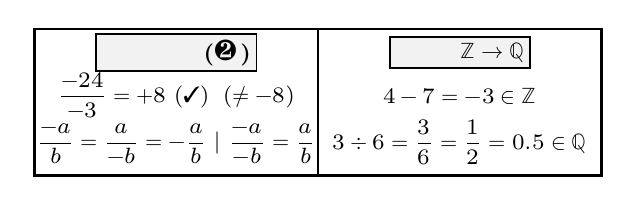
\begin{tikzpicture}[scale=1.0, every node/.style={font=\footnotesize, text=black}]
  \draw[black, line width=0.9pt] (0,0) rectangle (7.20, 1.86);
  \draw[black, line width=0.8pt] (3.60,0) -- (3.60,1.86);
  % Box Left: Sign closure
  \node[fill=headgray, inner sep=2pt, draw=black, line width=0.6pt] at (1.80, 1.56) {\textbf{ប្រយ័ត្នសញ្ញាដក (\cnum{2})}};
  \node at (1.80, 1.02) {$\dfrac{-24}{-3} = +8$ \en{(\ding{51})} \;($\neq -8$)};
  \node at (1.80, 0.40) {$\dfrac{-a}{b} = \dfrac{a}{-b} = -\dfrac{a}{b}$ \textbar\ $\dfrac{-a}{-b} = \dfrac{a}{b}$};
  % Box Right: Integer closure -> Rational
  \node[fill=headgray, inner sep=2pt, draw=black, line width=0.6pt] at (5.40, 1.56) {\textbf{ការបង្កើត $\mathbb{Z} \to \mathbb{Q}$}};
  \node[align=center] at (5.40, 1.00) {$4 - 7 = -3 \in \mathbb{Z}$};
  \node[align=center] at (5.40, 0.42) {$3 \div 6 = \dfrac{3}{6} = \dfrac{1}{2} = 0.5 \in \mathbb{Q}$};
\end{tikzpicture}}

% ២. E1 Engage: បេសកកម្មសហគមន៍កំពង់ស្វាយ (ចែកស្រូវ & បញ្ជីបំណុល)
\newcommand{\figEngageRN}{%
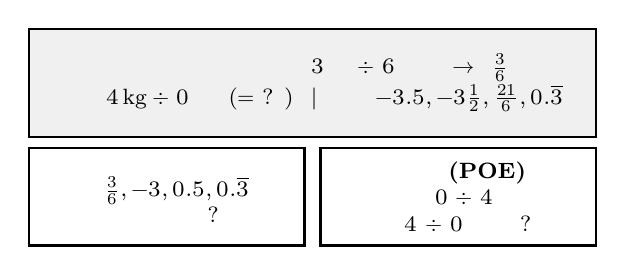
\begin{tikzpicture}[scale=1.0, every node/.style={font=\footnotesize, text=black}]
  \draw[black, line width=0.95pt, fill=panelgray] (0, 1.38) rectangle (7.20, 2.75);
  \node[align=center, text width=6.95cm] at (3.60, 2.065) {%
    \textbf{ទីផ្សារសហគមន៍កំពង់ស្វាយ}៖ ស្រូវ $3$ បាវ $\div$ $6$ គ្រួសារ $\to \frac{3}{6}$\\
    ផ្លែឈើ $4\unit{kg} \div 0$ នាក់ ($=$ ? ) \;\textbar{}\; បញ្ជី៖ $-3.5,-3\frac{1}{2},\frac{21}{6},0.\overline{3}$};
  % Bottom 2 prompt boxes
  \draw[black, line width=0.85pt] (0, 0) rectangle (3.50, 1.24);
  \node[align=center, text width=3.25cm] at (1.75, 0.62) {\textbf{សំណួរទី ១៖}\\ តើ $\frac{3}{6},-3,0.5,0.\overline{3}$\\ ជាក្រុមតែមួយឬទេ?};
  \draw[black, line width=0.85pt] (3.70, 0) rectangle (7.20, 1.24);
  \node[align=center, text width=3.25cm] at (5.45, 0.62) {\textbf{សំណួរទី ២ (\en{POE})៖}\\ ហេតុអ្វី $0\div 4$ មានន័យ\\ តែ $4\div 0$ គ្មានន័យ?};
\end{tikzpicture}}

% ៣. E2 Act 1: ជញ្ជាំងបន្ទះបត់ 1:1 & បន្ទាត់ចំនួនភ្លោះ [-1.5, +1.5]
\newcommand{\figFoldStripRN}{%
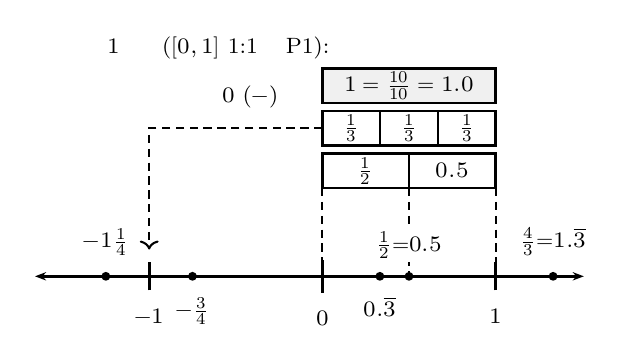
\begin{tikzpicture}[scale=1.0, every node/.style={font=\footnotesize, text=black}]
  % 1 unit = 2.20 cm, x=3.80 is 0 -> -1 is 1.60, +1 is 6.00, -1.5 is 0.50, +1.5 is 7.10
  \node[anchor=west] at (0.05, 3.86) {\textbf{ជញ្ជាំងបត់ $1$ ឯកតា} ($[0,1]$ \en{1:1} លើ \en{P1}):};
  % Row 1: Whole [3.80..6.00]
  \draw[black, line width=0.95pt, fill=panelgray] (3.80, 3.16) rectangle (6.00, 3.60);
  \node at (4.90, 3.38) {$1 = \frac{10}{10} = 1.0$};
  % Row 2: Thirds (NO vertical drop crosses through this strip!)
  \draw[black, line width=0.95pt] (3.80, 2.62) rectangle (4.533, 3.06);
  \draw[black, line width=0.95pt] (4.533, 2.62) rectangle (5.267, 3.06);
  \draw[black, line width=0.95pt] (5.267, 2.62) rectangle (6.00, 3.06);
  \node at (4.167, 2.84) {$\frac{1}{3}$};
  \node at (4.900, 2.84) {$\frac{1}{3}$};
  \node at (5.633, 2.84) {$\frac{1}{3}$};
  % Row 3 (bottom): Halves so middle drop at 4.90 drops straight down cleanly
  \draw[black, line width=0.95pt] (3.80, 2.08) rectangle (4.90, 2.52);
  \draw[black, line width=0.95pt] (4.90, 2.08) rectangle (6.00, 2.52);
  \node at (4.35, 2.30) {$\frac{1}{2}$};
  \node at (5.45, 2.30) {$0.5$};

  % Drop dashed alignment strictly BELOW bottom strip
  \draw[black, densely dashed, line width=0.7pt] (3.80, 2.08) -- (3.80, 0.96);
  \draw[black, densely dashed, line width=0.7pt] (4.90, 2.08) -- (4.90, 0.96);
  \draw[black, densely dashed, line width=0.7pt] (6.00, 2.08) -- (6.00, 0.96);

  % Left reflection brace cleanly separated from strip wall
  \draw[black, densely dashed, line width=0.75pt, ->] (3.80, 2.84) -- (1.60, 2.84) -- (1.60, 1.30);
  \node[fill=white, inner sep=1pt] at (2.40, 3.24) {ត្រឡប់ឆ្វេង $0$ ($-$)};

  % Twin Number Line [-1.5, +1.5] at y = 0.96
  \draw[{Stealth[length=4pt]}-{Stealth[length=4pt]}, black, line width=1.1pt] (0.15, 0.96) -- (7.12, 0.96);
  \draw[black, line width=1.1pt] (1.60, 0.78) -- (1.60, 1.14);
  \node[below=3pt] at (1.60, 0.78) {$-1$};
  \draw[black, line width=1.2pt] (3.80, 0.75) -- (3.80, 1.17);
  \node[below=3pt] at (3.80, 0.75) {$0$};
  \draw[black, line width=1.1pt] (6.00, 0.78) -- (6.00, 1.14);
  \node[below=3pt] at (6.00, 0.78) {$1$};

  % Target rational numbers nicely alternated above/below with ZERO overlaps
  \fill[black] (1.05, 0.96) circle (1.6pt);
  \node[above=4pt] at (1.05, 0.96) {$-1\frac{1}{4}$};
  \fill[black] (2.15, 0.96) circle (1.6pt);
  \node[below=4pt] at (2.15, 0.96) {$-\frac{3}{4}$};
  \fill[black] (4.53, 0.96) circle (1.6pt);
  \node[below=4pt] at (4.53, 0.96) {$0.\overline{3}$};
  \fill[black] (4.90, 0.96) circle (1.6pt);
  \node[above=4pt, fill=white, inner sep=1pt] at (4.90, 1.00) {$\frac{1}{2}{=}0.5$};
  \fill[black] (6.73, 0.96) circle (1.6pt);
  \node[above=4pt] at (6.73, 0.96) {$\frac{4}{3}{=}1.\overline{3}$};
\end{tikzpicture}}

% ៤. E2 Act 2: Dual POE (លេខ 0 និងកត្តាបឋម {2,5} + សញ្ញាចម្រុះដក)
\newcommand{\figDualPOERN}{%
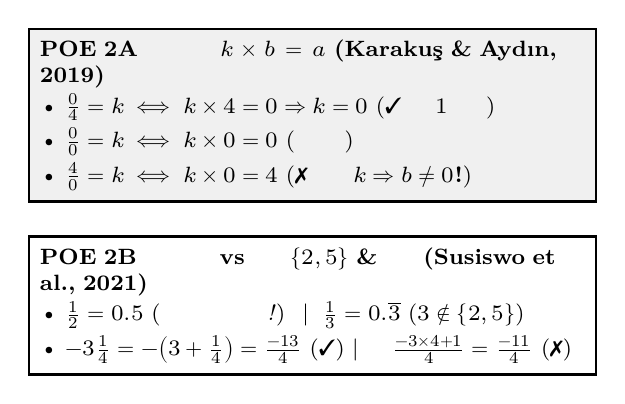
\begin{tikzpicture}[scale=1.0, every node/.style={font=\footnotesize, text=black}]
  \node[anchor=north west, draw=black, line width=0.9pt, fill=panelgray, inner sep=4pt, align=left, text width=6.92cm] at (0, 4.42) {%
    \textbf{POE 2A៖ ច្រាសផលគុណ $k \times b = a$ (\en{Karakuş \& Aydın, 2019})}\\[1.5pt]
    \textbullet\ $\frac{0}{4}=k \iff k\times 4=0 \Rightarrow k=0$ (\ding{51} មាន $1$ តម្លៃ)\\[1.5pt]
    \textbullet\ $\frac{0}{0}=k \iff k\times 0=0$ (មិនកំណត់)\\[1.5pt]
    \textbullet\ $\frac{4}{0}=k \iff k\times 0=4$ (\ding{55} \textbf{គ្មាន $k \Rightarrow b\neq 0$!})};

  \node[anchor=south west, draw=black, line width=0.9pt, fill=white, inner sep=4pt, align=left, text width=6.92cm] at (0, 0) {%
    \textbf{POE 2B៖ បឋមនឹងគ្នា vs កត្តា $\{2,5\}$ \& សញ្ញា (\en{Susiswo et al., 2021})}\\[1.5pt]
    \textbullet\ $\frac{1}{2}=0.5$ (\textit{បឋមនឹងគ្នា តែដាច់!}) \;\textbar{}\; $\frac{1}{3}=0.\overline{3}$ ($3 \notin \{2,5\}$)\\[1.5pt]
    \textbullet\ $-3\frac{1}{4} = -\!\left(3+\frac{1}{4}\right) = \frac{-13}{4}$ (\ding{51}) \textbar\ \textbf{ហាម} $\frac{-3\times 4+1}{4}=\frac{-11}{4}$ (\ding{55})};
\end{tikzpicture}}

% ៥. E3 Explain: Hub-and-Spoke 5 ទម្រង់ + ផលគុណខ្វែង ad=bc
\newcommand{\figHubSpokeRN}{%
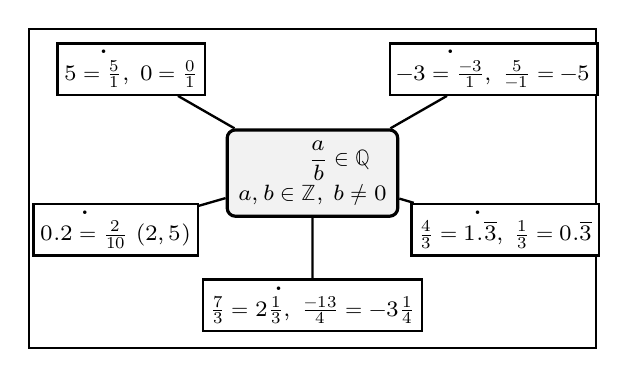
\begin{tikzpicture}[scale=1.0, every node/.style={font=\footnotesize, text=black}]
  \draw[black, line width=0.95pt] (0,0) rectangle (7.20, 4.05);
  % Hub in center
  \node[draw=black, line width=1.15pt, fill=headgray, rounded corners=3pt, inner sep=4pt, align=center] (HUB) at (3.60, 2.22) {\textbf{ស្នូល៖ } $\dfrac{a}{b}\in\mathbb{Q}$\\ $a,b\in\mathbb{Z},\; b\neq 0$};
  % 5 Spokes cleanly spaced
  \node[draw=black, line width=0.8pt, fill=white, inner sep=2.5pt, align=center] (S1) at (1.30, 3.54) {\textbf{១. ចំនួនគត់}\\ $5 = \frac{5}{1},\; 0 = \frac{0}{1}$};
  \node[draw=black, line width=0.8pt, fill=white, inner sep=2.5pt, align=center] (S2) at (5.90, 3.54) {\textbf{២. គត់រ៉ឺឡាទីបដក}\\ $-3=\frac{-3}{1},\; \frac{5}{-1}=-5$};
  \node[draw=black, line width=0.8pt, fill=white, inner sep=2.5pt, align=center] (S3) at (1.10, 1.50) {\textbf{៣. ទសភាគដាច់}\\ $0.2=\frac{2}{10}$ ($2,5$)};
  \node[draw=black, line width=0.8pt, fill=white, inner sep=2.5pt, align=center] (S4) at (6.05, 1.50) {\textbf{៤. ទសភាគខួប}\\ $\frac{4}{3}=1.\overline{3},\; \frac{1}{3}=0.\overline{3}$};
  \node[draw=black, line width=0.8pt, fill=white, inner sep=2.5pt, align=center] (S5) at (3.60, 0.54) {\textbf{៥. ចំនួនចំរុះ}\\ $\frac{7}{3}=2\frac{1}{3},\; \frac{-13}{4}=-3\frac{1}{4}$};
  \draw[black, line width=0.85pt] (HUB) -- (S1) (HUB) -- (S2) (HUB) -- (S3) (HUB) -- (S4) (HUB) -- (S5);
\end{tikzpicture}}

% ៦. E4 Elaborate: [tracing] គំរូទី១ (កែ 3.5=21/6) និងផលគុណខ្វែង គំរូទី២
\newcommand{\figModelTracingRN}{%
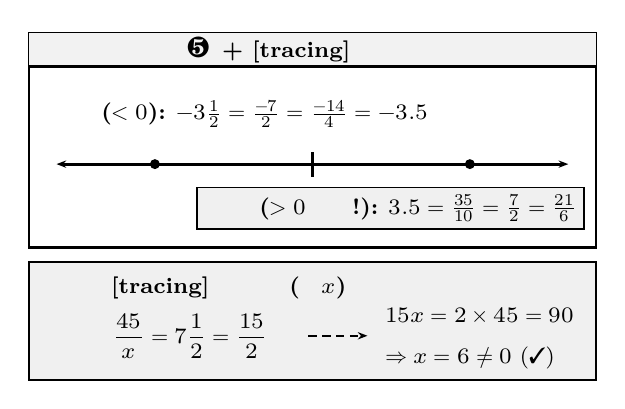
\begin{tikzpicture}[scale=1.0, every node/.style={font=\footnotesize, text=black}]
  \draw[black, line width=0.9pt] (0, 1.68) rectangle (7.20, 4.40);
  \fill[headgray] (0, 3.98) rectangle (7.20, 4.40);
  \draw[black, line width=0.8pt] (0, 3.98) -- (7.20, 3.98);
  \node[anchor=west] at (0.12, 4.19) {\textbf{គំរូទី ១៖ បំបែកសញ្ញា \cnum{5} + \en{[tracing]} ទាំង ២ ក្រុម}};
  \draw[{Stealth[length=3.5pt]}-{Stealth[length=3.5pt]}, black, line width=1.0pt] (0.35, 2.74) -- (6.85, 2.74);
  \draw[black, line width=1.05pt] (3.60, 2.58) -- (3.60, 2.90);
  \node[below=2pt] at (3.60, 2.58) {$0$};
  \fill[black] (1.60, 2.74) circle (1.8pt);
  \node[anchor=west, align=left, inner sep=2pt] at (0.14, 3.38) {\textbf{ក្រុម ១ ($<0$):} $-3\frac{1}{2}=\frac{-7}{2}=\frac{-14}{4}=-3.5$};
  \fill[black] (5.60, 2.74) circle (1.8pt);
  \node[anchor=east, fill=panelgray, draw=black, line width=0.5pt, inner sep=2.5pt, align=left] at (7.06, 2.18) {\textbf{ក្រុម ២ ($>0$ កែខ្វះ!):} $3.5 = \frac{35}{10} = \frac{7}{2} = \frac{21}{6}$};

  % Bottom: Ex 2 cross-mult tracing
  \draw[black, line width=0.9pt, fill=panelgray] (0, 0) rectangle (7.20, 1.50);
  \node[anchor=north west] at (0.14, 1.43) {\textbf{គំរូទី ២ \en{[tracing]} ផលគុណខ្វែង (រក $x$)៖}};
  \node at (2.05, 0.56) {$\dfrac{45}{x} = 7\dfrac{1}{2} = \dfrac{15}{2}$};
  \draw[-{Stealth[length=3.5pt]}, black, densely dashed, line width=0.85pt] (3.55, 0.56) -- (4.30, 0.56);
  \node[anchor=west] at (4.40, 0.82) {$15x = 2\times 45 = 90$};
  \node[anchor=west] at (4.40, 0.28) {$\Rightarrow x = 6 \neq 0$ (\ding{51})};
\end{tikzpicture}}

% ៧. E5 Evaluate: កាតវិនិច្ឆ័យ A-D 2x2 (ប្រយុទ្ធអន្ទាក់ ០, ទសភាគខួប, Negz, សញ្ញា)
\newcommand{\figExitCardsRN}{%
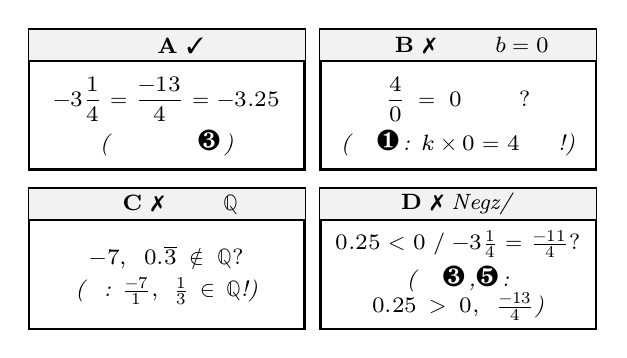
\begin{tikzpicture}[scale=1.0, every node/.style={font=\footnotesize, text=black}]
  % Card A (Top-Left)
  \draw[black, line width=0.9pt] (0, 2.02) rectangle (3.50, 3.80);
  \fill[headgray] (0, 3.40) rectangle (3.50, 3.80);
  \draw[black, line width=0.8pt] (0, 3.40) -- (3.50, 3.40);
  \node at (1.75, 3.60) {\textbf{កាត \en{A} \ding{51}}};
  \node[align=center, text width=3.20cm] at (1.75, 2.70) {$-3\dfrac{1}{4} = \dfrac{-13}{4} = -3.25$\\[2pt] \textit{(ត្រឹមត្រូវតាម \cnum{3})}};

  % Card B (Top-Right)
  \draw[black, line width=0.9pt] (3.70, 2.02) rectangle (7.20, 3.80);
  \fill[headgray] (3.70, 3.40) rectangle (7.20, 3.80);
  \draw[black, line width=0.8pt] (3.70, 3.40) -- (7.20, 3.40);
  \node at (5.45, 3.60) {\textbf{កាត \en{B} \ding{55}} \textit{អន្ទាក់ $b=0$}};
  \node[align=center, text width=3.20cm] at (5.45, 2.70) {$\dfrac{4}{0} = 0$ ជាសនិទាន?\\[2pt] \textit{(ខុស \cnum{1}: $k\times 0 = 4$ គ្មាន!)}};

  % Card C (Bottom-Left)
  \draw[black, line width=0.9pt] (0, 0) rectangle (3.50, 1.78);
  \fill[headgray] (0, 1.38) rectangle (3.50, 1.78);
  \draw[black, line width=0.8pt] (0, 1.38) -- (3.50, 1.38);
  \node at (1.75, 1.58) {\textbf{កាត \en{C} \ding{55}} \textit{កាត់ចោល $\mathbb{Q}$}};
  \node[align=center, text width=3.20cm] at (1.75, 0.68) {$-7,\; 0.\overline{3} \notin \mathbb{Q}$?\\[2pt] \textit{(ខុស: $\frac{-7}{1},\; \frac{1}{3}\in\mathbb{Q}$!)}};

  % Card D (Bottom-Right)
  \draw[black, line width=0.9pt] (3.70, 0) rectangle (7.20, 1.78);
  \fill[headgray] (3.70, 1.38) rectangle (7.20, 1.78);
  \draw[black, line width=0.8pt] (3.70, 1.38) -- (7.20, 1.38);
  \node at (5.45, 1.58) {\textbf{កាត \en{D} \ding{55}} \textit{Negz/ចំរុះ}};
  \node[align=center, text width=3.35cm] at (5.45, 0.68) {$0.25<0$ / $-3\frac{1}{4}=\frac{-11}{4}$?\\[2pt] \textit{(ខុស \cnum{3},\cnum{5}: $0.25>0,\;\frac{-13}{4}$)}};
\end{tikzpicture}}

% ៨. ជំហានទី៥ កិច្ចការផ្ទះ៖ រាប់សញ្ញាដក #1 & ពិនិត្យកត្តាបឋម #4(ង)
\newcommand{\figHWRN}{%
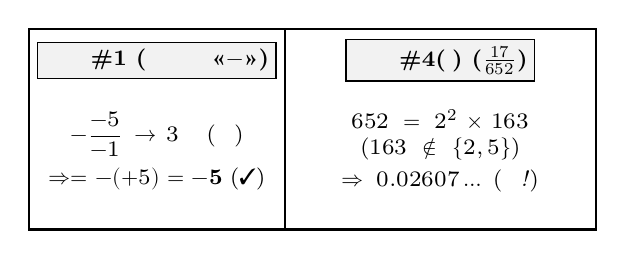
\begin{tikzpicture}[scale=1.0, every node/.style={font=\footnotesize, text=black}]
  \draw[black, line width=0.9pt] (0,0) rectangle (7.20, 2.55);
  \draw[black, line width=0.8pt] (3.25,0) -- (3.25,2.55);
  \node[fill=headgray, inner sep=2.5pt, draw=black, line width=0.6pt] at (1.625, 2.15) {\textbf{គន្លឹះ \en{\#1} (រាប់សញ្ញា «$-$»)}};
  \node[align=center, text width=3.00cm] at (1.625, 1.00) {$-\dfrac{-5}{-1} \to 3$ ដក (សេស)\\[3pt] $\Rightarrow = -(+5) = \mathbf{-5}$ (\ding{51})};
  \node[fill=headgray, inner sep=2.5pt, draw=black, line width=0.6pt] at (5.225, 2.15) {\textbf{គន្លឹះ \en{\#4}(ង) ($\frac{17}{652}$)}};
  \node[align=center, text width=3.70cm] at (5.225, 1.00) {$652 = 2^2 \times 163$\\ ($163 \notin \{2,5\}$)\\[2pt] $\Rightarrow 0.02607\dots$ (\textit{ខួប!})};
\end{tikzpicture}}

% ============================================================================
% ចាប់ផ្ដើមឯកសារ (Document Body — ទំព័រ 1..N-1 ពេញ >=90%, អាស្រ័យតាមខ្លឹមសារ 4–8+ ទំព័រ)
% ============================================================================
\begin{document}
\fontsize{10pt}{15.2pt}\selectfont

% -------------------- ក្បាលកិច្ចតែងការ (Header) --------------------
\begin{center}
  {\muol\fontsize{11pt}{16pt}\selectfont ព្រះរាជាណាចក្រកម្ពុជា}\\[2pt]
  {\muol\fontsize{10pt}{15pt}\selectfont ជាតិ សាសនា ព្រះមហាក្សត្រ}\\[1pt]
  \khmflourish
\end{center}

\vspace{-15pt}
{\muol\fontsize{9.5pt}{13.2pt}\selectfont
មន្ទីរអប់រំ យុវជន និងកីឡា ខេត្តកំពង់ធំ\\
ការិយាល័យអប់រំ យុវជន និងកីឡា ស្រុកកំពង់ស្វាយ\\
អនុវិទ្យាល័យព្រះក្រសាំង}

\vspace{2pt}
\begin{center}
  {\muol\fontsize{10pt}{15pt}\selectfont កិច្ចតែងការបង្រៀន}
\end{center}
\vspace{1pt}

% -------------------- ព័ត៌មានទូទៅ (Metadata) --------------------
{\renewcommand{\arraystretch}{1.06}
\hspace*{4.2cm}%
\begin{tabular}{@{}l l l@{}}
  - \hspace{0.35cm} មុខវិជ្ជា & : & គណិតវិទ្យា ថ្នាក់ទី៨ (ពីជគណិត) \\
  - \hspace{0.35cm} ចំណងជើងមេរៀន & : & មេរៀនទី១ ចំនួនសនិទាន \\
  - \hspace{0.35cm} ចំណងជើងរង & : & ១. សញ្ញាណចំនួនសនិទាន (ទំ.១--២ \& លំហាត់ ទំ.១១) \\
  - \hspace{0.35cm} រយៈពេល & : & ១ ម៉ោងសិក្សា (៥០ នាទី) \\
  - \hspace{0.35cm} បង្រៀនដោយ & : & ហុក ប៊ុនថែន \\
  - \hspace{0.35cm} កាលបរិច្ឆេទ & : & ថ្ងៃចន្ទ ទី២ ខែវិច្ឆិកា ឆ្នាំ២០២៦ \\
\end{tabular}

\vspace{2pt}

% -------------------- I. វត្ថុបំណង --------------------
\textbf{I.} {\muol វត្ថុបំណង}\\[2pt]
\hspace*{0.55cm}%
\begin{tabular}{@{}l l L{14.0cm}@{}}
  \wcirc \hspace{0.25cm} វិជ្ជាសម្បទា & : & សិស្សកំណត់និយមន័យចំនួនសនិទាន $\frac{a}{b}\;(a,b\in\mathbb{Z},\; b\neq 0)$, រៀបរាប់ទម្រង់ទាំង ៥ (ចំនួនគត់ គត់រ៉ឺឡាទីប ទសភាគ ទសភាគខួប ចំនួនចំរុះ) និងប្រាប់វិធាន $\frac{a}{b}=\frac{c}{d} \Leftrightarrow ad=bc\;(b,d\neq 0)$ ។ \\
  \wcirc \hspace{0.25cm} បំណិនសម្បទា & : & សិស្សបត់បន្ទះក្រដាស \en{1:1} បម្លែងទម្រង់ឆ្លាស់គ្នា រួមទាំងសញ្ញាចម្រុះដក ($-3\frac{1}{4}$), បំពេញចន្លោះ $3.5=\frac{21}{6}$ និងរកអញ្ញាត $x=6$, $(x,y)=(10,-1)$ តាម \textbf{[tracing]} និង \cnum{1}--\cnum{5} ។ \\
  \wcirc \hspace{0.25cm} ចរិយាសម្បទា & : & សហការក្នុង «ក្រុមវិស្វករសហគមន៍» តាមវិន័យ \en{Pause-Ask / Pause-Review} ដោយប្រុងប្រយ័ត្នសញ្ញាដក និងលក្ខខណ្ឌ $b\neq 0$ ដោយហេតុផលច្បាស់លាស់ ។ \\
\end{tabular}

\vspace{2pt}

% -------------------- II. សម្ភារៈឧបទេស --------------------
\textbf{II.} {\muol សម្ភារៈឧបទេស}\\[2pt]
\hspace*{0.55cm}$\bullet$ \hspace{0.35cm} សៀវភៅគោលគណិតវិទ្យាថ្នាក់ទី៨ (ទំ.១--២, ១១) បន្ទាត់ក្រិត \en{cm} កន្ត្រៃ ខ្មៅដៃ \textbf{[tracing]} និងកញ្ចប់ \en{B\&W} (\en{P1 1:1}--\en{P6})

\vspace{2pt}

% -------------------- III. វិធីសាស្រ្តបង្រៀន --------------------
\textbf{III.} {\muol វិធីសាស្រ្តបង្រៀន}\\[2pt]
\hspace*{0.55cm}%
\begin{tabular}{@{}l l L{13.8cm}@{}}
  $\bullet$ \hspace{0.35cm} គោលវិធី & : \hspace{0.7cm} & សិស្សមជ្ឈមណ្ឌល \\
  $\bullet$ \hspace{0.35cm} យុទ្ធវិធីបង្រៀន & : & ស្ថាបនានិយម គម្រូ \en{5Es} (បត់ក្រដាស \en{1:1} ផ្ទៀងបន្ទាត់ភ្លោះ, \en{Dual POE}, \en{Hub-and-Spoke}, \textbf{[tracing]}, \en{Relay 3} តួនាទី) \\
\end{tabular}
}

\vspace{2pt}

% -------------------- IV. ដំណើរការបង្រៀន --------------------
\textbf{IV.} {\muol ដំណើរការបង្រៀន}

\vspace{-3pt}

% ============================================================================
% តារាងដំណើរការបង្រៀន (Granular 2-4 line Sub-rows + Dedicated Figure Rows)
% ============================================================================
\renewcommand{\arraystretch}{1.15}
\begin{longtable}{|L{5.50cm}|L{7.90cm}|L{4.80cm}|}
\hline
\rowcolor{headgray}
\multicolumn{1}{|c|}{\muol សកម្មភាពគ្រូ} &
\multicolumn{1}{c|}{\muol ខ្លឹមសារមេរៀន} &
\multicolumn{1}{c|}{\muol សកម្មភាពសិស្ស} \\
\hline
\endfirsthead

\hline
\endhead

\hline
\endfoot

\hline
\endlastfoot

% ==================== ជំហានទី១ (2min) ====================
\stepheader{ជំហានទី១ \enbf{(}រដ្ឋបាលថ្នាក់\enbf{)}}
$\bullet$ គ្រូពិនិត្យអវត្តមាន និងអនាម័យថ្នាក់\par\vspace{2pt}
$\bullet$ គ្រូរៀបក្រុម ៣ នាក់ («ក្រុមវិស្វករសហគមន៍»)\par\vspace{2pt}
$\bullet$ ចែកកញ្ចប់ \en{P1 (1:1)} ដាក់ផ្កាប់មុខលើតុ
&
\textbf{រដ្ឋបាលថ្នាក់៖}\par\vspace{2pt}
-- ពិនិត្យអវត្តមាន និងសុវត្ថិភាពកន្ត្រៃ/បន្ទាត់\par\vspace{2pt}
-- ត្រៀមក្រុមពិសោធន៍ ១:១ (៣ នាក់/ក្រុម)
&
$\circ$ ប្រធានថ្នាក់រាយការណ៍អវត្តមាន\par\vspace{2pt}
$\circ$ សិស្សអង្គុយតាមក្រុម ៣ នាក់\par\vspace{2pt}
$\circ$ រៀបចំបន្ទាត់ កន្ត្រៃ និងខ្មៅដៃ \\[3pt]
\hline

% ==================== ជំហានទី២ (9min: <=3 + 3 + E1 3) ====================
\stepheader{ជំហានទី២ \enbf{(}ត្រួតពិនិត្យមូលដ្ឋាន \enbf{+} ទំនាក់ទំនងមេរៀនថ្មី\enbf{)}}
% --- ២.១ ត្រួតពិនិត្យមេរៀនមុន/មូលដ្ឋានទី៧ (<=3min) ---
\ditem \textbf{ពិនិត្យមូលដ្ឋានថ្នាក់ទី៧} \timenote{($\le 3\unit{min}$)}\par\vspace{2pt}
$\bullet$ គ្រូសរសេរលំហាត់រហ័ស៖ $4-7$, $\frac{-24}{-3}$, $3\div 6$\par\vspace{2pt}
-- សំណួរ៖ «តើ $\frac{-24}{-3}$ ស្មើ $8$ ឬ $-8$? ហេតុអ្វី?» \timenote{(រហ័ស $\le 3'$)}
&
\textbf{មូលដ្ឋានចំនួនគត់រ៉ឺឡាទីប និងប្រភាគ៖}\par\vspace{2pt}
$7 - 4 = 3 \in \mathbb{N}$ \quad តែ \quad $4 - 7 = -3 \in \mathbb{Z}$\par\vspace{2pt}
$6 \div 3 = 2 \in \mathbb{Z}$ \quad តែ \quad $3 \div 6 = \dfrac{3}{6} = \dfrac{1}{2}$\par\vspace{2pt}
$\dfrac{-24}{-3} = +8$ (ដកចែកដក បានបូក)
&
$\circ$ សិស្សគិតផ្ទៀងចម្លើយរហ័ស\par\vspace{2pt}
$\circ$ ឆ្លើយ៖ «$4-7=-3\in\mathbb{Z}$; $\frac{-24}{-3}=8$ ព្រោះដកចែកដកបានបូក!» \\[3pt]
& \cfig{\figSignCheckRN} & \\[3pt]

% --- ២.២ រំលឹកមេរៀនទាក់ទង (3min) ---
\ditem \textbf{រំលឹកមេរៀនទាក់ទង} \timenote{(3min)}\par\vspace{2pt}
$\bullet$ គ្រូសួររំលឹកទម្រង់សញ្ញាប្រភាគ និងទសភាគពីថ្នាក់ទី៧៖\par\vspace{2pt}
\hspace*{0.3em}-- សំណួរ៖ «តើ $0.5$ សរសេរជាប្រភាគមានភាគបែង $10$ ដូចម្ដេច? ចុះ $-\frac{5}{1}$ ស្មើប៉ុន្មាន?»
&
\textbf{រំលឹកទម្រង់មូលដ្ឋាន (ទំ.១)៖}\par\vspace{2pt}
-- ចំនួនគត់៖ $5 = \dfrac{5}{1}$, \quad $-5 = \dfrac{-5}{1} = \dfrac{5}{-1} = -\dfrac{5}{1}$\par\vspace{2pt}
-- ទសភាគដប់៖ $0.2 = \dfrac{2}{10}$, \quad $0.5 = \dfrac{5}{10} = \dfrac{1}{2}$
&
$\circ$ សិស្សឆ្លើយព្រមៗគ្នា៖\par\vspace{2pt}
«$0.5=\frac{5}{10}=\frac{1}{2}$; $-\frac{5}{1}=-5$!» \\[3pt]

% --- ២.៣ E1 - Engage (3min) ---
\fiveE{E1 - Engage} \timenote{(3min)}\par\vspace{2pt}
$\bullet$ គ្រូលើកបេសកកម្ម «ទីផ្សារសហគមន៍កំពង់ស្វាយ» លើក្ដារខៀន\par\vspace{2pt}
\hspace*{0.3em}-- សំណួរ ១៖ «តើ $3\div 6$, $-3$, $0.5$, និង $0.\overline{3}$ ជារបស់ក្រុមតែមួយឬទេ?»
&
\textbf{បេសកកម្ម E1៖ ទីផ្សារសហគមន៍កំពង់ស្វាយ}\par\vspace{2pt}
កសិករច្រូតស្រូវ $3$ បាវចែក $6$ គ្រួសារ ($3\div 6$), ផ្លែឈើ $4\unit{kg}$ ចែក $0$ នាក់ ($4\div 0$)
&
$\circ$ សិស្សសង្កេតស្ថានភាព\par\vspace{2pt}
$\circ$ ក្រុមបញ្ចេញយោបល់ទស្សន៍ទាយខុសៗគ្នា \\[3pt]

\hspace*{0.3em}-- សំណួរ ២៖ «ហេតុអ្វី $0\div 4$ ចែកបាន តែ $4\div 0$ ហាមចែក?» \timenote{(ស្រង់ការទាយ — កុំទាន់ប្រាប់ចម្លើយ)}
&
និងបញ្ជីបំណុល៖ $-3.5,\; -3\frac{1}{2},\; \frac{21}{6},\; 0.\overline{3}$ ។
&
$\circ$ ត្រៀមចង់ដឹងចម្លើយពិតក្នុង \fiveE{E2} \\[3pt]
& \cfig{\figEngageRN} & \\[3pt]
\hline

% ==================== ជំហានទី៣ (17min: E2 11m + E3 6m) ====================
\stepheader{ជំហានទី៣ \enbf{(}ខ្លឹមសារមេរៀនថ្មី\enbf{)}}
% --- ៣.១ ចំណងជើង & E2 Act 1 (6min) ---
$\bullet$ គ្រូសរសេរចំណងជើងមេរៀនលើក្ដារខៀន\par\vspace{2pt}
\fiveE{E2 - Explore} \timenote{(11min)}\par\vspace{2pt}
\ditem \textbf{សកម្មភាព ១៖ បត់បន្ទះ 1:1 លើបន្ទាត់ភ្លោះ} \timenote{(6min)}
&
មេរៀនទី១ {\muol ចំនួនសនិទាន}\par\vspace{2pt}
\textbf{១. សញ្ញាណចំនួនសនិទាន}\par\vspace{2pt}
\textbf{សកម្មភាព ១ (\en{P1 1:1})៖} ដាក់បន្ទះ $1$ ឯកតា ($6.00\unit{cm}$) លើ $[0, 1]$ និង $[0, -1]$
&
$\circ$ សិស្សកត់ចំណងជើងមេរៀន\par\vspace{2pt}
$\circ$ ផ្ទៀងបន្ទាត់ $5.00\unit{cm}$ និងកាត់បន្ទះ \\[3pt]

$\bullet$ គ្រូណែនាំផ្ទៀងក្រិត $5.00\unit{cm}$ លើសន្លឹក \en{P1 (Actual Size 100\%)}\par\vspace{2pt}
$\bullet$ ឱ្យក្រុមកាត់បន្ទះ $1$ ឯកតា ($=6.00\unit{cm}$) បត់ជា $2$, $3$, $4$ ផ្នែកស្មើ រួចផ្ទៀងលើបន្ទាត់ $[-1.5, +1.5]$
&
-- បត់ $2$ ស្មើ $\to \frac{1}{2} = 0.5 = \frac{5}{10} = \frac{3}{6}$\par\vspace{2pt}
-- បត់ $3$ ស្មើ $\to \frac{1}{3} = 0.\overline{3}$ និង $\frac{4}{3} = 1\frac{1}{3} = 1.\overline{3}$\par\vspace{2pt}
-- ឆ្លុះខាងឆ្វេង $0$ ($-$): $-\frac{3}{4}=-0.75,\; -1\frac{1}{4}=-\frac{5}{4}$
&
$\circ$ បត់រក $\frac{1}{2}=0.5$ និង $\frac{1}{3}$ លើបន្ទាត់ភ្លោះ\par\vspace{2pt}
$\circ$ ដៅទីតាំងអវិជ្ជមានខាងឆ្វេង $0$ \\[3pt]
& \cfig{\figFoldStripRN} & \\[3pt]

% --- ៣.២ E2 Act 2 Dual POE (5min) ---
\ditem \textbf{សកម្មភាព ២៖ \en{Dual POE} អន្ទាក់គំនិត} \timenote{(5min)}\par\vspace{2pt}
$\bullet$ \textbf{POE 2A (អន្ទាក់សូន្យ)៖} សួរទាយ $\frac{0}{4}$, $\frac{4}{0}$, $\frac{0}{0}$ រួចសាករក $k$ តាម $k\times b = a$
&
\textbf{សកម្មភាព ២៖ ការផ្ទៀងផ្ទាត់ \en{POE 2A}៖}\par\vspace{2pt}
-- $\frac{0}{4}=k \iff k\times 4=0 \Rightarrow k=0$ (\ding{51});\par\vspace{2pt}
$\frac{4}{0}=k \iff k\times 0=4$ (គ្មាន $k$ $\Rightarrow$ គ្មានន័យ! $b\neq 0$)
&
$\circ$ សិស្សទាយ និងពន្យល់មូលហេតុ $k\times 0=4$ មិនពិត\par\vspace{2pt}
$\circ$ ទាញលក្ខខណ្ឌ $b\neq 0$ \\[3pt]

$\bullet$ \textbf{POE 2B (ទសភាគខួប \& សញ្ញា)៖}\par\vspace{2pt}
\hspace*{0.3em}-- សំណួរ ១៖ «$\frac{1}{2}$ បឋមនឹងគ្នាដែរ ហេតុអ្វី $=0.5$ ដាច់?»
&
-- \textbf{\en{POE 2B} (កត្តា $\{2,5\}$)៖} $\frac{a}{b}$ សម្រួលរួច ដាច់ $\iff$ $b$ មានតែកត្តាបឋម $\{2,5\}$ ។
&
$\circ$ សង្កេតកត្តា $\{2,5\}$ ទល់ $3$ \\[3pt]

\hspace*{0.3em}-- សំណួរ ២៖ «$-3\frac{1}{4}$ ស្មើ $\frac{-13}{4}$ ឬ $\frac{-11}{4}$?»
&
-- $-3\frac{1}{4} = -\left(3+\frac{1}{4}\right) = \frac{-13}{4}$ (ឆ្វេង $-3$ បន្ថែម $\frac{1}{4}$ មិនមែន $\frac{-11}{4}$)
&
$\circ$ ទាញច្បាប់សញ្ញាចម្រុះដក \\[3pt]
& \cfig{\figDualPOERN} & \\[3pt]

% --- ៣.៣ E3 Explain: និយមន័យ + Hub-and-Spoke 5 ទម្រង់ ---
\fiveE{E3 - Explain} \timenote{(6min)}\par\vspace{2pt}
$\bullet$ គ្រូដឹកនាំសិស្សបង្គុំនិយមន័យផ្លូវការ និងដ្យាក្រាម \en{Hub-and-Spoke} ៥ ទម្រង់ (ផ្ទាំង \en{P4})\par\vspace{2pt}
\hspace*{0.3em}-- សំណួរ៖ «ហេតុអ្វី $-3$, $0.5$, $0.\overline{3}$ និង $-3\frac{1}{4}$ សុទ្ធតែស្ថិតក្នុង $\mathbb{Q}$?»
&
\textbf{និយមន័យ (ទំ.១)៖}\par\vspace{2pt}
\grayparbox{ចំនួនសនិទានជាចំនួនដែលមានទម្រង់ $\dfrac{a}{b}$ ដែល $a, b \in \mathbb{Z}$ និង $b \neq 0$ ។}\par\vspace{2pt}
-- ដូចនេះ $-3, 0, 0.5, \frac{-2}{3}, 4\frac{1}{5}, 2.\overline{3}$ សុទ្ធតែជាចំនួនសនិទាន ($\mathbb{Q}$) ។
&
$\circ$ សិស្សរួមគ្នាអាន និងសង្ខេបនិយមន័យ $\frac{a}{b}\;(b\neq 0)$\par\vspace{2pt}
$\circ$ ភ្ជាប់ទម្រង់ទាំង ៥ តាម \en{Hub-and-Spoke} \\[3pt]
& \cfig{\figHubSpokeRN} & \\[3pt]

% --- ៣.៤ E3 Explain: វិធានស្មើគ្នា ad=bc & Warrant Bank ①–⑤ ---
$\bullet$ គ្រូបង្ហាញវិធានផលគុណខ្វែង (ទំ.២ ដោយបន្ថែម $b,d\neq 0$)\par\vspace{2pt}
$\bullet$ បិទផ្ទាំង \textbf{ធនាគារហេតុផល \cnum{1}--\cnum{5}} (ទំព័រ ៤) ជាសំអាងវិភាគ
&
\textbf{វិធានសមភាពចំនួនសនិទាន (ទំ.២ កែលម្អលក្ខខណ្ឌ)៖}\par\vspace{2pt}
\grayparbox{ជាទូទៅ៖ ចំពោះ $b\neq 0,\; d\neq 0$៖ $\dfrac{a}{b} = \dfrac{c}{d} \iff ad = bc$ ។}\par\vspace{2pt}
\textbf{ធនាគារហេតុផល \cnum{1}--\cnum{5}៖}\par\vspace{2pt}
\cnum{1} និយមន័យ $\frac{a}{b}\;(b\neq 0)$ \;\textbar{}\; \cnum{2} ច្បាប់សញ្ញា $-\frac{a}{b}=\frac{-a}{b}=\frac{a}{-b}$, $\frac{-a}{-b}=\frac{a}{b}$\par\vspace{2pt}
\cnum{3} បម្លែងទម្រង់ $5$ យ៉ាង \;\textbar{}\; \cnum{4} ផលគុណខ្វែង $ad=bc$ \;\textbar{}\; \cnum{5} សញ្ញាឆ្វេង/ស្ដាំ $0$
&
$\circ$ សិស្សកត់វិធាន $ad=bc\;(b,d\neq 0)$\par\vspace{2pt}
$\circ$ ផ្ទៀងផ្ទាំង \cnum{1}--\cnum{5} ទំព័រ ៤ \\[3pt]
\hline

% ==================== ជំហានទី៤ (20min: E4 10m + E5 10m) ====================
\stepheader{ជំហានទី៤ \enbf{(}ពង្រីកចំណេះដឹង\enbf{)}}
% --- ៤.១ E4 Elaborate: លំហាត់គំរូទី ១ & ២ (ទំ.២) + [tracing] ---
\fiveE{E4 - Elaborate} \timenote{(10min)}\par\vspace{2pt}
$\bullet$ ចែកកាត \textbf{«៣ ជំហានស៊ើបអង្កេត»} (ទំព័រ ២)
&
{\muol លំហាត់គំរូទី \enbf{1}} \textbf{(ទំ.២ កែបំពេញ)៖}\par\vspace{2pt}
ចូរផ្គុំចំនួនស្មើគ្នា៖ $-3\frac{1}{2},\; 3.5,\; \frac{-7}{2},\; \frac{-14}{4},\; -3.5,\; \frac{21}{6}$ ។
&
$\circ$ សិស្សទទួលកាត \en{P2} (\en{2-up})\par\vspace{2pt}
$\circ$ ត្រៀមខ្មៅដៃ \textbf{[tracing]} \\[3pt]

\hspace*{0.3em}\cnum{1} ចែកក្រុមសញ្ញា ($<0$ vs $>0$) ដោយ \textbf{[tracing]}
&
\textbf{ដំណោះស្រាយ \en{[tracing]}៖}\par\vspace{2pt}
-- ក្រុមអវិជ្ជមាន ($<0$)៖ $-3\frac{1}{2} = \frac{-7}{2} = \frac{-14}{4} = -3.5$ (\cnum{3}, \cnum{5})
&
$\circ$ សិស្សគូសអូស \textbf{[tracing]} ញែកក្រុម\par\vspace{2pt}
$\circ$ កត់ក្រុមអវិជ្ជមាន \\[3pt]

\hspace*{0.3em}\cnum{2} បម្លែងជា $\frac{a}{b}$ រួម — \timenote{បង្ហាញក្រុម $3.5=\frac{21}{6}$ ដែលសៀវភៅភ្លេច!}\par\vspace{2pt}
\hspace*{0.3em}\cnum{3} បញ្ជាក់ក្រុមវិជ្ជមានបំពេញសៀវភៅខ្វះ
&
-- ក្រុមវិជ្ជមាន ($>0$ \textbf{បំពេញសៀវភៅខ្វះ!})៖\par\vspace{2pt}
$3.5 = \frac{35}{10} = \frac{7}{2} = \frac{21}{6}$
&
$\circ$ រកឃើញក្រុមទី ២ ($3.5=\frac{21}{6}$) បន្ថែមលើសៀវភៅ \\[3pt]
& \cfig{\figModelTracingRN} & \\[3pt]

$\bullet$ គ្រូដឹកនាំលំហាត់គំរូទី ២ តាម ៣ ជំហាន
&
{\muol លំហាត់គំរូទី \enbf{2}} \textbf{(ទំ.២)៖} កំណត់ $x$ ដើម្បីឱ្យ $\dfrac{45}{x}$ ស្មើ $7\dfrac{1}{2}$ ។\par\vspace{2pt}
\textbf{ចម្លើយ៖}\par\vspace{2pt}
-- បម្លែង $7\frac{1}{2}=\frac{15}{2} \Rightarrow \frac{45}{x}=\frac{15}{2}$ ($x\neq 0$, \cnum{1})\par\vspace{2pt}
-- គុណខ្វែង៖ $15x = 2\times 45 = 90$ (\cnum{4}) $\Rightarrow$ \graybox{$x = 6$} ។
&
$\circ$ សិស្សដោះស្រាយតាមជំហាន $x=6$ \\[3pt]

$\bullet$ សួរ \textbf{EIA Looking-Back (\en{30s})}៖\par\vspace{2pt}
\hspace*{0.3em}-- សំណួរ ១៖ «ហេតុអ្វី $-3\frac{1}{2} = -\frac{7}{2}$ មិនមែន $-\frac{5}{2}$?»\par\vspace{2pt}
\hspace*{0.3em}-- សំណួរ ២៖ «ហេតុអ្វីត្រូវផ្គុំ $3.5=\frac{21}{6}$ ផង?»
&
\textbf{សំយោគ \en{EIA}៖}\par\vspace{2pt}
១) $-3\frac{1}{2} = -\left(3+\frac{1}{2}\right) = \frac{-7}{2}$ (\cnum{3})\par\vspace{2pt}
២) $3.5=\frac{21}{6}$ ជាគូវិជ្ជមានដែលសៀវភៅភ្លេច
&
$\circ$ ឆ្លើយ EIA៖ «$-3\frac{1}{2}=-(3+\frac{1}{2})$ និងកុំទុក $3.5, \frac{21}{6}$ ចោល!» \\[3pt]

% --- ៤.២ E5 Evaluate: Relay 3 តួនាទី (ប្រតិបត្តិ + សញ្ញាដក) ---
\fiveE{E5 - Evaluate} \timenote{(10min)}\par\vspace{2pt}
\ditem \textbf{ភាគទី ១៖ \en{Relay 3} តួនាទី (\en{5min}, ទំព័រ ៣)} \timenote{(Pause-Ask / Review)}\par\vspace{2pt}
\hspace*{0.3em}\cnum{1} \textbf{តួនាទី ១ (\en{Pause-Ask})៖} \en{[tracing]} $-0.2=\frac{-1}{5}$ និងពិនិត្យ $x\neq 0$\par\vspace{2pt}
\hspace*{0.3em}\cnum{2} \textbf{តួនាទី ២៖} គណនា $x, y$ តាម \cnum{4} ក្នុង «ប្រតិបត្តិ»
&
{\muol ប្រតិបត្តិ} \textbf{(ទំ.២)៖} រក $x, y$ ដើម្បីឱ្យ $\frac{-2}{x},\; \frac{y}{5},\; -0.2$ ស្មើគ្នា។\par\vspace{2pt}
-- $-0.2 = \frac{-2}{10} = \frac{-1}{5}$ (\cnum{3})\par\vspace{2pt}
-- $\frac{-2}{x}=\frac{-1}{5} \Rightarrow x = 10\neq 0$ (\cnum{4}); \quad $\frac{y}{5}=\frac{-1}{5} \Rightarrow y = -1$ (\cnum{4})
&
$\circ$ ក្រុមអនុវត្តតួនាទី ១ និង ២ ប្ដូរវេនគ្នា\par\vspace{2pt}
$\circ$ ផ្ទៀង $x=10,\; y=-1$ \\[3pt]

\hspace*{0.3em}\cnum{3} \textbf{តួនាទី ៣ (\en{Pause-Review})៖} រាប់សញ្ញាដក $-\frac{-5}{-1}$ និង \textbf{បិទ E1}
&
-- តេស្តសញ្ញា៖ $-\frac{-5}{-1} = -5$ ($3$ ដកសេស, \cnum{2})\par\vspace{2pt}
\textbf{បិទ E1៖} $3\div 6, -3, 0.5, 0.\overline{3} \in \mathbb{Q}$ តែ $4\div 0$ ហាម ($b\neq 0$)!
&
$\circ$ តួនាទី ៣ បញ្ជាក់សញ្ញា និងបិទបេសកកម្ម \fiveE{E1} \\[3pt]

% --- ៤.៣ E5 Evaluate: កាត A-D & សំបុត្រចេញ 3 សំណួរ ---
\ditem \textbf{ភាគទី ២៖ កាត \en{A--D} \& សំបុត្រចេញ (\en{5min}, ទំព័រ ៥)}\par\vspace{2pt}
$\bullet$ បង្ហាញកាត \en{A--D} ឱ្យសិស្សលើក \ding{51}/\ding{55} និងកែខុស
&
\textbf{កាតវិនិច្ឆ័យ \en{A--D}៖}\par\vspace{2pt}
-- \textbf{A} (\ding{51}): $-3\frac{1}{4}=\frac{-13}{4}=-3.25$ \;\textbar{}\; \textbf{B} (\ding{55}): $\frac{4}{0}$ គ្មានន័យ (\cnum{1})\par\vspace{2pt}
-- \textbf{C} (\ding{55}): $-7, 0.\overline{3}\in\mathbb{Q}$ \;\textbar{}\; \textbf{D} (\ding{55}): $0.25>0,\; \frac{-13}{4}$
&
$\circ$ សិស្សលើក \ding{51} (A) និង \ding{55} (B, C, D) ព្រមទាំងកែខុស \\[3pt]

$\bullet$ ឱ្យសិស្សបំពេញសំបុត្រចេញ ៣ សំណួរ (\en{60--90s})
&
\textbf{សំបុត្រចេញ៖}\par\vspace{2pt}
១) $-2\frac{3}{4} = \frac{-11}{4} = -2.75$ \quad ២) $\frac{0}{-5}=0\in\mathbb{Q}$ តែ $\frac{-5}{0}$ គ្មានន័យ\par\vspace{2pt}
៣) $\frac{12}{m}=-0.6=\frac{-3}{5} \Rightarrow m = -20$ ។
&
$\circ$ សរសេរសំបុត្រចេញប្រគល់គ្រូ \\[3pt]
& \cfig{\figExitCardsRN} & \\[3pt]
\hline

% ==================== ជំហានទី៥ (<=2min) ====================
\stepheader{ជំហានទី៥ \enbf{(}កិច្ចការផ្ទះ \enbf{+} បណ្ដាំផ្ញើ\enbf{)}}
\timenote{ចំណាយពេលឱ្យតិចបំផុតកុំឱ្យលើស 2min}\par\vspace{2pt}
$\bullet$ ចែកប័ណ្ណកិច្ចការផ្ទះ (ទំព័រ ៦) ពីសៀវភៅគោល ទំ.១១\par\vspace{2pt}
$\bullet$ រំលឹកវិធីរាប់សញ្ញាដកលើ \textbf{\#1} និងកត្តាបឋម $652$ លើ \textbf{\#4(ង)}\par\vspace{2pt}
$\bullet$ បណ្ដាំផ្ញើ៖ អានជាមុន \textbf{២.១ ការប្រៀបធៀបចំនួនសនិទាន (ទំ.២–៣)}
&
\centerline{\muol កិច្ចការផ្ទះ \enbf{(}ទំ\enbf{.}១១\enbf{)}}\par\vspace{2pt}
\textbf{\#1:} រកចំនួនស្មើ $-5$ ក្នុង $\frac{-5}{1},\frac{5}{1},\frac{5}{-1},-\frac{5}{1},\frac{-5}{-1},-\frac{-5}{1},-\frac{-5}{-1}$\par\vspace{2pt}
\textbf{\#3:} សរសេរជាប្រភាគ៖ \textbf{ក.} $28.45$ \;\textbar{}\; \textbf{គ.} $1\frac{19}{50}$\par\vspace{2pt}
\textbf{\#4:} សរសេរជាទសភាគ៖ \textbf{ក.} $\frac{7}{100}$, \textbf{ខ.} $\frac{13}{10,000}$, \textbf{គ.} $\frac{3}{2^4}$, \textbf{ឃ.} $\frac{7}{2^3\cdot 5}$, \textbf{ង.} $\frac{17}{652}$
&
$\circ$ សិស្សកត់ត្រា និងទទួលប័ណ្ណកិច្ចការផ្ទះ\par\vspace{2pt}
$\circ$ ចាប់ផ្ដើមពិនិត្យសញ្ញាដក\par\vspace{2pt}
$\circ$ បាទ/ចាស៎លោកគ្រូ \\[3pt]
& \cfig{\figHWRN} & \\[3pt]
\end{longtable}

% -------------------- កាលបរិច្ឆេទ និងហត្ថលេខា (Date & Signature) --------------------
\vspace{2pt}
\hfill
\begin{minipage}{9.8cm}
  {\centering
    ថ្ងៃចន្ទ ៨រោច ខែអស្សុជ ឆ្នាំមមី អដ្ឋស័ក ពុទ្ធសករាជ ២៥៧០\\[2pt]
    កំពង់ស្វាយ, ថ្ងៃទី២ ខែវិច្ឆិកា ឆ្នាំ២០២៦\\[3pt]
    {\muol គ្រូបង្រៀន}\par}
  \vspace{32pt}
  \hfill{\muol ហុក ប៊ុនថែន}\hspace*{1.4cm}
\end{minipage}

\end{document}
